\documentclass[english,11pt]{beamer}

\DeclareMathOperator{\Cov}{Cov}
\DeclareMathOperator{\Var}{Var}
\DeclareMathOperator{\E}{\mathbb{E}}
\DeclareMathOperator{\Proba}{\mathbb{P}}

\newcommand{\Covb}[2]{\ensuremath{\Cov\!\left[#1,#2\right]}}
\newcommand{\Eb}[1]{\ensuremath{\E\!\left[#1\right]}}
\newcommand{\Pb}[1]{\ensuremath{\Proba\!\left[#1\right]}}
\newcommand{\Varb}[1]{\ensuremath{\Var\!\left[#1\right]}}

% norm
\newcommand{\norm}[1]{\| #1 \|}

\newcommand{\indep}{\rotatebox[origin=c]{90}{$\models$}}





\usepackage{mathptmx,amsmath,amssymb,graphicx,bibentry,bbm,babel,ragged2e}

\makeatletter

\newcommand{\noun}[1]{\textsc{#1}}
\newcommand{\jitem}[1]{\item \begin{justify} #1 \end{justify} \vfill{}}
\newcommand{\sframe}[2]{\frame{\frametitle{#1} #2}}

\newenvironment{centercolumns}{\begin{columns}[c]}{\end{columns}}
%\newenvironment{jitem}{\begin{justify}\begin{itemize}}{\end{itemize}\end{justify}}

\usetheme{Warsaw}
\setbeamertemplate{footline}[text line]{}
\setbeamercolor{structure}{fg=purple!50!blue, bg=purple!50!blue}

\setbeamersize{text margin left=15pt,text margin right=15pt}

\setbeamercovered{transparent}


\@ifundefined{showcaptionsetup}{}{%
 \PassOptionsToPackage{caption=false}{subfig}}
\usepackage{subfig}

\usepackage[utf8]{inputenc}
\usepackage[T1]{fontenc}

\usepackage{multirow}


\makeatother

\begin{document}





\title{Spatial sensitivity analysis of social simulation models}

\author{J.~Raimbault$^{1,2,3,4,\ast}$ and J. Perret$^{1}$\\
\texttt{$\ast$ juste.raimbault@ign.fr}
}


\institute{$^{1}$LASTIG, IGN-ENSG\\
$^{2}$CASA, UCL\\
$^{3}$UPS CNRS 3611 ISC-PIF\\
$^{4}$UMR CNRS 8504 G{\'e}ographie-cit{\'e}s
}


\date{CCS 2023\\\smallskip
Online session - Auditorium 2\\\smallskip
October 17th 2023
}

\frame{\maketitle}





\section{Spatial sensitivity analysis: state-of-the-art}


\sframe{Validation of simulation models}{


Typology of \textbf{validation methods for simulation models} from a systematic review \cite{raimbault2023validation}

\begin{columns}
	\begin{column}{0.49\textwidth}
		\begin{itemize}
	   \item prediction
	   \item sensitivity analysis
	   \item uncertainty
	   \item multiple methods
	   \item benchmark
	   \item calibration
	   \item optimisation
\end{itemize}
	\end{column}
	\begin{column}{0.49\textwidth}
		\begin{itemize}
	   \item visualisation
	   \item Pattern Oriented Modelling
	   \item participatory
	   \item exploration
	   \item mixed
	   \item surrogate
\end{itemize}
	\end{column}
\end{columns}

\medskip

Methods, standards and definitions strongly depend on disciplines and model functions \cite{raimbault2019validation}

}




\sframe{Specificities of socio-spatial systems}{

\justify

$\rightarrow$ Spatio-temporal non-stationarity and non-ergodicity \cite{raimbault2019urban}
$\rightarrow$ Fuzzy and noisy data \cite{olteanu2015knowledge}
$\rightarrow$ Genericity/specificity of patterns and processes \cite{raimbault2020empowering}
$\rightarrow$ Modifiable Areal Unit Problem \cite{wong2004modifiable}
$\rightarrow$ Multiscalar systems \cite{raimbault2021strong}

% Wong, D. (2009). The modifiable areal unit problem (MAUP). The SAGE handbook of spatial analysis, 105, 23.

% \textit{Processes specific to scales, coupling implies dedicated ontologies} \cite{raimbault:halshs-02351722}

% \textit{Spatial non-stationarity of road network properties} \cite{raimbault2019urban}

%\textit{Urban systems are simultaneously universal and particular} \cite{raimbault2020empowering}

}




\sframe{Spatial sensitivity analysis}{

% Spatial simulation models for socio-technical systems re- quire a thorough validation process in order to obtain action- able policy insights from their application. While the sensi- tivity to model parameters is usually well accounted for, it was shown recently by [1] that the variability of model out- puts due to the spatial configuration could be as much as the variability due to model parameters, with an investigation on classical socio-spatial models such as the Schelling model. A scala library implementing generators of synthetic urban configurations at different scales (district, urban area, system of cities) was developed in that context [2]. Indeed, testing the effect of the spatial configuration can be done by sam- pling synthetic realistic urban systems for which the model phase space is obtained and compared.

\textbf{Spatial configurations are model parameters too}

\medskip

\begin{itemize}
	\item ``\textit{Space matters}'': impact of spatial configuration on model behavior
	\item Model behaviours which are robust to spatial configuration
	\item Model behaviours which are robust to noise in real datasets
\end{itemize}

\medskip

$\implies$ \textit{\textbf{Construction of a generic library for spatial sensitivity analysis, including the generation of synthetic data, perturbation of real data and indicators}}


% This contribution proposes to summarise different ongo- ing streams of research extending and developing this new crucial component of the validation of socio-spatial simulation models.

 
}


\sframe{Synthetic data: general context}{

\justify

$\rightarrow$ coupling models with spatial configuration generators (spatial synthetic data) gives model sensitivity to space through sensitivity analysis of the coupled model

\bigskip

$\rightarrow$ synthetic urban forms resembling real configurations

\bigskip

$\rightarrow$ at different scales: microscopic (buildings), mesoscopic (population distribution), macroscopic (system of cities)

}



\sframe{Synthetic building layouts}{

\textit{At the microscopic scale (district): generating building layouts}

\nocite{raimbault2019generating}

\medskip

Raimbault, J., \& Perret, J. (2019, July). Generating urban morphologies at large scales. In Artificial Life Conference Proceedings (pp. 179-186). MIT Press.

\medskip

\begin{itemize}
	\item systematic comparison of simple processual generators
	\item introduction of morphological indicators
	\item calibration on sampled layouts from OpenStreetMap
\end{itemize}

}





\sframe{Synthetic population grids}{

\textit{At the mesoscopic scale: population grids}

\medskip


\begin{itemize}
	\item a reaction-diffusion model for population distributions
	\item urban form measures at the mesoscopic scale
	\item synthetic generators coupling population and road networks
\end{itemize}


\bigskip
\bigskip

\footnotesize

Raimbault, J. (2018). Calibration of a density-based model of urban morphogenesis. PloS one, 13(9), e0203516.

\nocite{raimbault2018calibration}

\smallskip

Raimbault, J. (2019). An urban morphogenesis model capturing interactions between networks and territories. In The Mathematics of Urban Morphology (pp. 383-409). Birkhäuser, Cham.

\nocite{raimbault2019urban}


}



\sframe{Synthetic systems of cities}{


\textit{At the macroscopic scale: synthetic systems of cities}


\begin{itemize}
	\item Evolutive urban theory: systems of cities follow general stylised facts \cite{pumain2018evolutionary}
	\item Rank-size law \cite{pumain2006evolutionary}
	\item Central place theory
\end{itemize}

\medskip

$\rightarrow$ \textit{Cities-network co-evolution model explored on synthetic systems of cities} \nocite{raimbault2021modeling}

Raimbault, J. (2021). Modeling the co-evolution of cities and networks. In Handbook of Cities and Networks (pp. 166-193). E. Elgar.


}





\sframe{Method flowchart}{

\textit{General workflow to test the spatial sensitivity of simulation models}

\bigskip

\footnotesize

Raimbault, J., Cottineau, C., Le Texier, M., Le Nechet, F., \& Reuillon, R. (2019). Space Matters: Extending Sensitivity Analysis to Initial Spatial Conditions in Geosimulation Models. Journal of Artificial Societies and Social Simulation, 22(4).

\bigskip

\centering

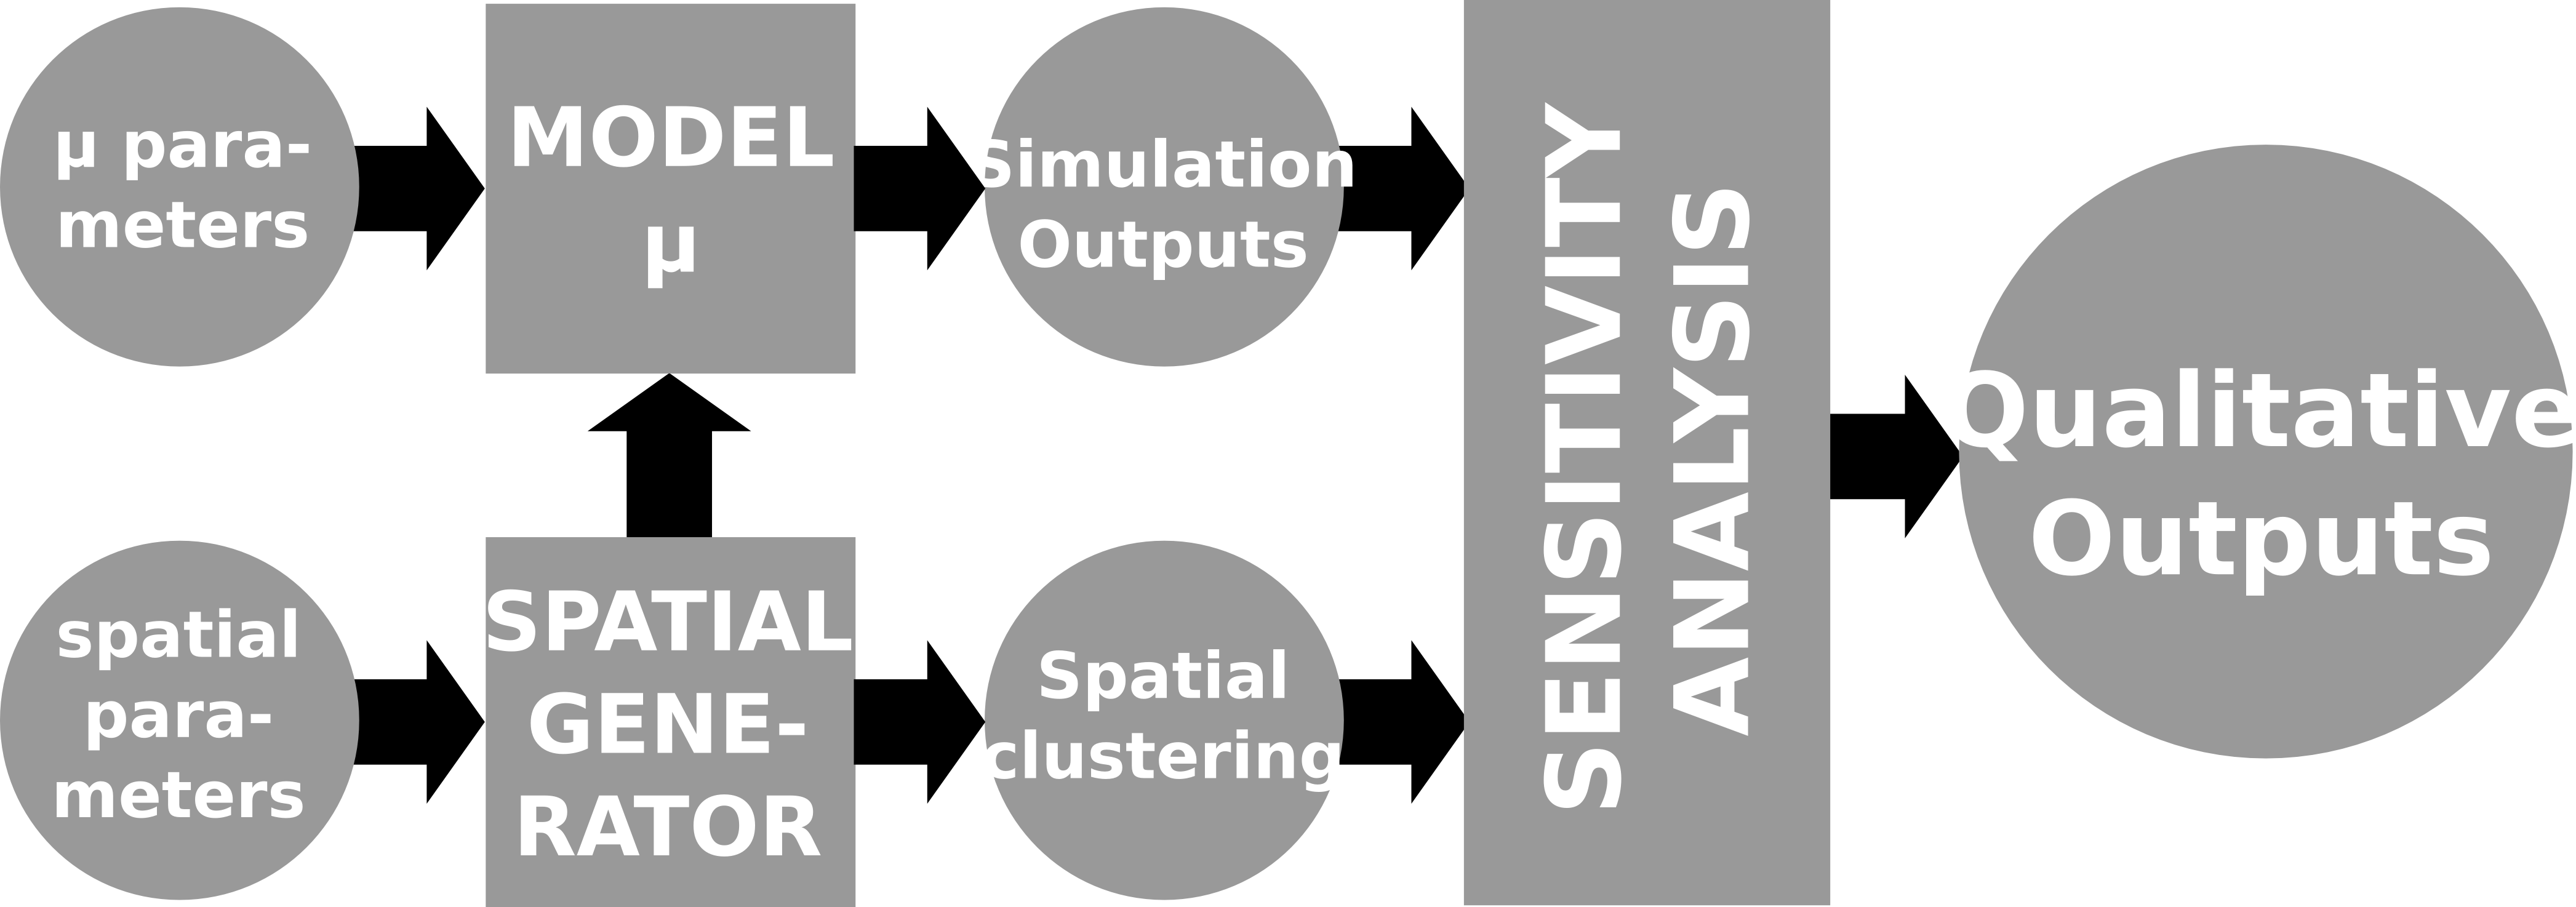
\includegraphics[width=\textwidth]{../../gisruk2020/communication/figures/spatialsens_spacemattersworkflow.png}

}




\sframe{Implementation: integration into OpenMOLE}{


Library implemented in \texttt{scala}: advantages of functional and object programming; Apache Spark; no widely used GIS library in scala.

\medskip

\url{https://github.com/openmole/spatialdata}

\medskip

$\rightarrow$ integration into the OpenMOLE model exploration open source software \cite{reuillon2013openmole}

\begin{center}

\includegraphics[height=0.13\textheight]{../../gisruk2020/communication/figures/logos/iconOM.png}

\includegraphics[height=0.13\textheight]{../../gisruk2020/communication/figures/logos/openmole.png}
\end{center}


\textit{Enables seamlessly (i) model embedding; (ii) access to HPC resources; (iii) exploration and optimization algorithms}

\medskip

\url{https://openmole.org/}

}


%\sframe{Implementation in OpenMOLE}{
% spatialsmapling syntax 
%\begin{center}
%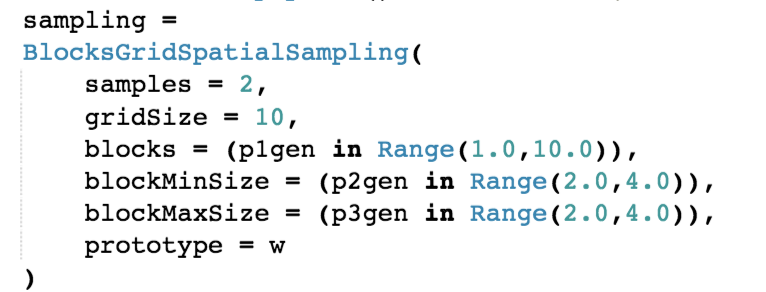
\includegraphics[width=0.8\textwidth]{figures/blocksampling.png}
%\end{center}
%\medskip
%\justify
%$\rightarrow$ other generators have their own primitives\\(\texttt{ExpMixtureThresholdSpatialSampling},\\ \texttt{PercolationGridSpatialSampling}) and arguments (\textbf{see the documentation})
%}







\section{Research directions}


\subsection{Benchmarking generators}

% First, the generator approach for synthetic urban config- urations was further explored. At the mesoscopic scale of an urban area, a benchmark of generative models for pop- ulation distribution was achieved, including models not in- vestigated before such as a gravity-based model [4] and a correlated percolation model [3]. Examples of generated configurations are shown in Fig. 1. A diversity-search al- gorithm provides the feasible morphological space for each model, showing the complementarity of the different generative processes to cover different regions of urban forms.

\sframe{}{

}




\subsection{Noise propagation and real data perturbation}



% Second, an approach based on noise propagation is being investigated [5], by exploring neighbour spatial configura- tions to existing ones. The main difficulty is to define small variations in the morphological space, as these do not fol- low standard distributions in most cases: for example in the case of a road network, moving uniformly or with a Gaus- sian noise coordinates of vertices will produce unrealistic configurations in terms of curvature. Similarly, angles of building polygons follow a very specific distribution with highly localised peaks. Some initial tests for generating re- alistic noises and linking these with the generative approach are being lead for building configurations.


\sframe{Real data perturbation}{


\medskip

$\rightarrow$ \textit{How does noise in real data impacts the result ?}


\medskip

\begin{itemize}
	\item Impact of missing elements
	\item Impact of imprecise coordinates or topology
	\item Optimal matching between spatial datasets
\end{itemize}


\bigskip

$\rightarrow$ \textit{How does perturbation of real data allows to explore scenario}

\medskip

\textbf{Examples:}

\begin{itemize}
   \item simulating urban projects by modifying population of areas with a given spatial correlation structure %Forcity example
	\item simulating network disruptions or new transportation lines
\end{itemize}


}



\subsection{Variance-based indicators}


% Third, the open issue of indicators to quantify the variability due to space is being tackled by introducing variance- based indicators following the classical approach by [6]. For a correct statistical estimation of such indicators, the sampling of the morphological space must have a high discrepancy, what is not ensured by simply sampling the parameter space of synthetic generators. An approach based on diversity search for these generators is being tested and compared to a parameter sampling, in the case of population distribution generators and the Schelling model.

\sframe{}{

}


\subsection{Interdisciplinary systematic review}


% Finally, the link with other fields in which model sensitiv- ity analysis and validation is much widely developed com- pared to computational social science, is investigated from a theoretical point of view. In environmental science, similar frameworks have been proposed such as the perturbation of spatial datasets described in [7].

\sframe{}{

\cite{koo2020position}

}









%\section{Discussion}

%\subsection{Indicators}
%\sframe{Spatial statistics}{
%\textit{In the spatial approach, spatial model indicators are also important: what% kind of spatial structure does the model produce ?}
%\bigskip 
% \begin{itemize}
% 	\item previous form indicators at different scales, applied on any spatialized variable or event: quantify level of aggregation, hierarchy, clustering
% 	\item spatial statistics indicators and methods
% 	\item more complicated approaches: fractals and multifractals, spatial datamining
% \end{itemize}
%}


\sframe{Discussion}{

% These complementary research axis contribute to a more robust validation process for socio-spatial simulation mod- els.


% morphogensis : interdisc ?

% suggest: ecology (habitat / spatial niches ?) ; topography ; ?

\textit{Developments}

\medskip

\begin{itemize}
	\item more spatial network generative models \cite{raimbault2018multi}, correlated synthetic data \cite{raimbault2019second}
	\item domain models: LUTI, urban dynamics
	\item other disciplines, ecology, geosciences \cite{mogheir2004characterizing}?
	\item interaction with data driven disciplines ? (planning, architecture, spatio-temporal datamining)
	\item genericity of some models? (reaction-diffusion)
	\item synthetic data generation methods (synthetic populations)
	\item synthetic data at the core of applied statistics methodology (less in spatial statistics?)
	\item port the library to more classic languages (python, R)
\end{itemize}


}






\sframe{Conclusion}{

\justify

$\rightarrow$ \textbf{Space matters: } relevance of spatially-explicit models and spatial sensitivity analysis.

\medskip

$\rightarrow$ \textbf{Synthetic data: } first experimental samplings included in OpenMOLE, soon more to come.

\medskip

$\rightarrow$ \textbf{Disciplinary context: } strong contingency on included models.

\bigskip
\bigskip

\textit{Get the library at } \url{https://github.com/openmole/spatialdata}

\medskip

\textit{Open issues at } \url{https://github.com/openmole/spatialdata/issues}

 

}




%%%%%%%%%%%%%%%%%%%%%
\begin{frame}[allowframebreaks]
\frametitle{References}
\bibliographystyle{apalike}
\bibliography{biblio}
\end{frame}
%%%%%%%%%%%%%%%%%%%%%%%%%%%%







\end{document}



\sframe{Synthesis of available tools}{



\begin{columns}
	\begin{column}{0.45\linewidth}
	
	\bigskip
	\bigskip
	
	Micro grid spatial samplings
	
	\medskip
	
	Meso grid spatial samplings
	
	\medskip
	
	Macro spatial samplings
	
	\medskip

	Spatial network generation
	
	\medskip

	Real data import
	
	\medskip

	Real data perturbations
	
	\medskip

	Spatial statistics
	
	\medskip

	Hybrid methods
	
	\medskip

	Domain models (transportation, land-use)
		
	\end{column}
	
	
	
	\begin{column}{0.2\linewidth}
		
		\vspace{-0.3cm}
		
		\textbf{OpenMOLE}
		
		\medskip
		
		{\textcolor{green}\cmark}
		
		\medskip
		
		{\textcolor{green}\cmark}
		
		\medskip
		
		{\textcolor{red}\xmark}
			
			\medskip
		
		{\textcolor{red}\xmark}
		
		\medskip
		
		{\textcolor{red}\xmark}
		
		\medskip
		
		{\textcolor{red}\xmark}
		
		\medskip

		{\textcolor{blue}\cmark}
		
		\medskip
		
		{\textcolor{red}\xmark}
		
		\medskip
		
		{\textcolor{red}\xmark}
			
	\end{column}
	
	
	
	\begin{column}{0.25\linewidth}
		
		\vspace{-0.3cm}
		
		\textbf{spatialdata}
		
		\medskip
		
		{\textcolor{green}\cmark}
		
		\medskip
		
		{\textcolor{green}\cmark}
		
		\medskip
		
		{\textcolor{green}\cmark}
			
			\medskip
		
		{\textcolor{blue}\cmark}
		
		\medskip
		
		{\textcolor{green}\xmark}
		
		\medskip
		
		{\textcolor{blue}\cmark}
		
		\medskip

		{\textcolor{blue}\cmark}
		
		\medskip
		
		{\textcolor{blue}\cmark}
		
		\medskip
		
		{\textcolor{blue}\cmark}
	\end{column}
	
		
	
	
\end{columns}



}





